% REV00 Tue 04 May 2021 13:55:16 WIB
% START Tue 04 May 2021 13:55:16 WIB

\chapter{XXX}

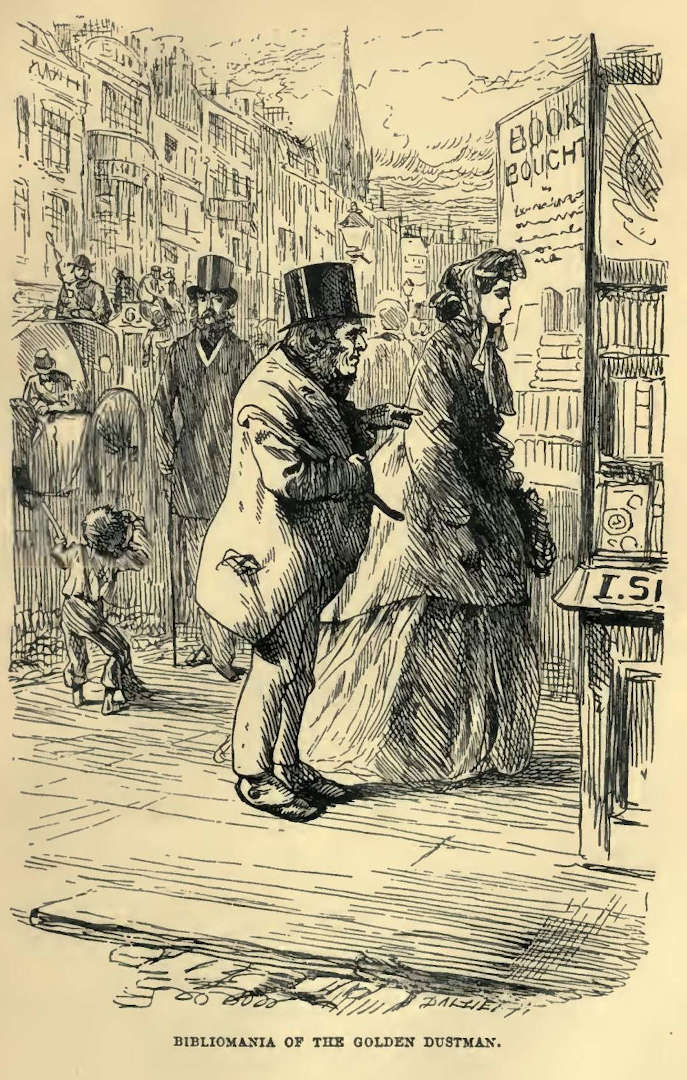
\includegraphics[scale=2.3]{03-05-01}

Chapter 7

BETTER TO BE ABEL THAN CAIN


Day was breaking at Plashwater Weir Mill Lock. Stars were yet visible,
but there was dull light in the east that was not the light of night.
The moon had gone down, and a mist crept along the banks of the river,
seen through which the trees were the ghosts of trees, and the water
was the ghost of water. This earth looked spectral, and so did the
pale stars: while the cold eastern glare, expressionless as to heat or
colour, with the eye of the firmament quenched, might have been likened
to the stare of the dead.

Perhaps it was so likened by the lonely Bargeman, standing on the brink
of the lock. For certain, Bradley Headstone looked that way, when a
chill air came up, and when it passed on murmuring, as if it
whispered something that made the phantom trees and water tremble--or
threaten--for fancy might have made it either.

He turned away, and tried the Lock-house door. It was fastened on the
inside.

‘Is he afraid of me?’ he muttered, knocking.

Rogue Riderhood was soon roused, and soon undrew the bolt and let him
in.

‘Why, T’otherest, I thought you had been and got lost! Two nights away!
I a’most believed as you’d giv’ me the slip, and I had as good as half a
mind for to advertise you in the newspapers to come for’ard.’

Bradley’s face turned so dark on this hint, that Riderhood deemed it
expedient to soften it into a compliment.

‘But not you, governor, not you,’ he went on, stolidly shaking his head.
‘For what did I say to myself arter having amused myself with that there
stretch of a comic idea, as a sort of a playful game? Why, I says to
myself; “He’s a man o’ honour.” That’s what I says to myself. “He’s a
man o’ double honour.”’

Very remarkably, Riderhood put no question to him. He had looked at him
on opening the door, and he now looked at him again (stealthily this
time), and the result of his looking was, that he asked him no question.

‘You’ll be for another forty on ‘em, governor, as I judges, afore you
turns your mind to breakfast,’ said Riderhood, when his visitor sat
down, resting his chin on his hand, with his eyes on the ground. And
very remarkably again: Riderhood feigned to set the scanty furniture in
order, while he spoke, to have a show of reason for not looking at him.

‘Yes. I had better sleep, I think,’ said Bradley, without changing his
position.

‘I myself should recommend it, governor,’ assented Riderhood. ‘Might you
be anyways dry?’

‘Yes. I should like a drink,’ said Bradley; but without appearing to
attend much.

Mr Riderhood got out his bottle, and fetched his jug-full of water,
and administered a potation. Then, he shook the coverlet of his bed and
spread it smooth, and Bradley stretched himself upon it in the clothes
he wore. Mr Riderhood poetically remarking that he would pick the bones
of his night’s rest, in his wooden chair, sat in the window as before;
but, as before, watched the sleeper narrowly until he was very sound
asleep. Then, he rose and looked at him close, in the bright daylight,
on every side, with great minuteness. He went out to his Lock to sum up
what he had seen.

‘One of his sleeves is tore right away below the elber, and the
t’other’s had a good rip at the shoulder. He’s been hung on to, pretty
tight, for his shirt’s all tore out of the neck-gathers. He’s been in
the grass and he’s been in the water. And he’s spotted, and I know with
what, and with whose. Hooroar!’

Bradley slept long. Early in the afternoon a barge came down. Other
barges had passed through, both ways, before it; but the Lock-keeper
hailed only this particular barge, for news, as if he had made a time
calculation with some nicety. The men on board told him a piece of news,
and there was a lingering on their part to enlarge upon it.

Twelve hours had intervened since Bradley’s lying down, when he got up.
‘Not that I swaller it,’ said Riderhood, squinting at his Lock, when he
saw Bradley coming out of the house, ‘as you’ve been a sleeping all the
time, old boy!’

Bradley came to him, sitting on his wooden lever, and asked what o’clock
it was? Riderhood told him it was between two and three.

‘When are you relieved?’ asked Bradley.

‘Day arter to-morrow, governor.’

‘Not sooner?’

‘Not a inch sooner, governor.’

On both sides, importance seemed attached to this question of relief.
Riderhood quite petted his reply; saying a second time, and prolonging a
negative roll of his head, ‘n--n--not a inch sooner, governor.’

‘Did I tell you I was going on to-night?’ asked Bradley.

‘No, governor,’ returned Riderhood, in a cheerful, affable, and
conversational manner, ‘you did not tell me so. But most like you meant
to it and forgot to it. How, otherways, could a doubt have come into
your head about it, governor?’

‘As the sun goes down, I intend to go on,’ said Bradley.

‘So much the more necessairy is a Peck,’ returned Riderhood. ‘Come in
and have it, T’otherest.’

The formality of spreading a tablecloth not being observed in Mr
Riderhood’s establishment, the serving of the ‘peck’ was the affair of
a moment; it merely consisting in the handing down of a capacious baking
dish with three-fourths of an immense meat pie in it, and the production
of two pocket-knives, an earthenware mug, and a large brown bottle of
beer.

Both ate and drank, but Riderhood much the more abundantly. In lieu of
plates, that honest man cut two triangular pieces from the thick crust
of the pie, and laid them, inside uppermost, upon the table: the one
before himself, and the other before his guest. Upon these platters he
placed two goodly portions of the contents of the pie, thus imparting
the unusual interest to the entertainment that each partaker scooped out
the inside of his plate, and consumed it with his other fare, besides
having the sport of pursuing the clots of congealed gravy over the plain
of the table, and successfully taking them into his mouth at last from
the blade of his knife, in case of their not first sliding off it.

Bradley Headstone was so remarkably awkward at these exercises, that the
Rogue observed it.

‘Look out, T’otherest!’ he cried, ‘you’ll cut your hand!’

But, the caution came too late, for Bradley gashed it at the instant.
And, what was more unlucky, in asking Riderhood to tie it up, and in
standing close to him for the purpose, he shook his hand under the smart
of the wound, and shook blood over Riderhood’s dress.

When dinner was done, and when what remained of the platters and what
remained of the congealed gravy had been put back into what remained of
the pie, which served as an economical investment for all miscellaneous
savings, Riderhood filled the mug with beer and took a long drink. And
now he did look at Bradley, and with an evil eye.

‘T’otherest!’ he said, hoarsely, as he bent across the table to touch
his arm. ‘The news has gone down the river afore you.’

‘What news?’

‘Who do you think,’ said Riderhood, with a hitch of his head, as if he
disdainfully jerked the feint away, ‘picked up the body? Guess.’

‘I am not good at guessing anything.’

‘She did. Hooroar! You had him there agin. She did.’

The convulsive twitching of Bradley Headstone’s face, and the sudden
hot humour that broke out upon it, showed how grimly the intelligence
touched him. But he said not a single word, good or bad. He only smiled
in a lowering manner, and got up and stood leaning at the window,
looking through it. Riderhood followed him with his eyes. Riderhood cast
down his eyes on his own besprinkled clothes. Riderhood began to have an
air of being better at a guess than Bradley owned to being.

‘I have been so long in want of rest,’ said the schoolmaster, ‘that with
your leave I’ll lie down again.’

‘And welcome, T’otherest!’ was the hospitable answer of his host. He had
laid himself down without waiting for it, and he remained upon the bed
until the sun was low. When he arose and came out to resume his journey,
he found his host waiting for him on the grass by the towing-path
outside the door.

‘Whenever it may be necessary that you and I should have any further
communication together,’ said Bradley, ‘I will come back. Good-night!’

‘Well, since no better can be,’ said Riderhood, turning on his heel,
‘Good-night!’ But he turned again as the other set forth, and added
under his breath, looking after him with a leer: ‘You wouldn’t be let to
go like that, if my Relief warn’t as good as come. I’ll catch you up in
a mile.’

In a word, his real time of relief being that evening at sunset, his
mate came lounging in, within a quarter of an hour. Not staying to fill
up the utmost margin of his time, but borrowing an hour or so, to be
repaid again when he should relieve his reliever, Riderhood straightway
followed on the track of Bradley Headstone.

He was a better follower than Bradley. It had been the calling of his
life to slink and skulk and dog and waylay, and he knew his calling
well. He effected such a forced march on leaving the Lock House that he
was close up with him--that is to say, as close up with him as he deemed
it convenient to be--before another Lock was passed. His man looked back
pretty often as he went, but got no hint of him. HE knew how to take
advantage of the ground, and where to put the hedge between them, and
where the wall, and when to duck, and when to drop, and had a thousand
arts beyond the doomed Bradley’s slow conception.

But, all his arts were brought to a standstill, like himself when
Bradley, turning into a green lane or riding by the river-side--a
solitary spot run wild in nettles, briars, and brambles, and encumbered
with the scathed trunks of a whole hedgerow of felled trees, on the
outskirts of a little wood--began stepping on these trunks and dropping
down among them and stepping on them again, apparently as a schoolboy
might have done, but assuredly with no schoolboy purpose, or want of
purpose.

‘What are you up to?’ muttered Riderhood, down in the ditch, and holding
the hedge a little open with both hands. And soon his actions made a
most extraordinary reply. ‘By George and the Draggin!’ cried Riderhood,
‘if he ain’t a going to bathe!’

He had passed back, on and among the trunks of trees again, and has
passed on to the water-side and had begun undressing on the grass. For
a moment it had a suspicious look of suicide, arranged to counterfeit
accident. ‘But you wouldn’t have fetched a bundle under your arm, from
among that timber, if such was your game!’ said Riderhood. Nevertheless
it was a relief to him when the bather after a plunge and a few strokes
came out. ‘For I shouldn’t,’ he said in a feeling manner, ‘have liked to
lose you till I had made more money out of you neither.’

Prone in another ditch (he had changed his ditch as his man had changed
his position), and holding apart so small a patch of the hedge that the
sharpest eyes could not have detected him, Rogue Riderhood watched the
bather dressing. And now gradually came the wonder that he stood up,
completely clothed, another man, and not the Bargeman.

‘Aha!’ said Riderhood. ‘Much as you was dressed that night. I see.
You’re a taking me with you, now. You’re deep. But I knows a deeper.’

When the bather had finished dressing, he kneeled on the grass, doing
something with his hands, and again stood up with his bundle under his
arm. Looking all around him with great attention, he then went to the
river’s edge, and flung it in as far, and yet as lightly as he could. It
was not until he was so decidedly upon his way again as to be beyond a
bend of the river and for the time out of view, that Riderhood scrambled
from the ditch.

‘Now,’ was his debate with himself ‘shall I foller you on, or shall I
let you loose for this once, and go a fishing?’ The debate continuing,
he followed, as a precautionary measure in any case, and got him again
in sight. ‘If I was to let you loose this once,’ said Riderhood then,
still following, ‘I could make you come to me agin, or I could find
you out in one way or another. If I wasn’t to go a fishing, others
might.--I’ll let you loose this once, and go a fishing!’ With that, he
suddenly dropped the pursuit and turned.

The miserable man whom he had released for the time, but not for long,
went on towards London. Bradley was suspicious of every sound he heard,
and of every face he saw, but was under a spell which very commonly
falls upon the shedder of blood, and had no suspicion of the real danger
that lurked in his life, and would have it yet. Riderhood was much
in his thoughts--had never been out of his thoughts since the
night-adventure of their first meeting; but Riderhood occupied a very
different place there, from the place of pursuer; and Bradley had been
at the pains of devising so many means of fitting that place to him, and
of wedging him into it, that his mind could not compass the possibility
of his occupying any other. And this is another spell against which
the shedder of blood for ever strives in vain. There are fifty doors by
which discovery may enter. With infinite pains and cunning, he double
locks and bars forty-nine of them, and cannot see the fiftieth standing
wide open.

Now, too, was he cursed with a state of mind more wearing and more
wearisome than remorse. He had no remorse; but the evildoer who can hold
that avenger at bay, cannot escape the slower torture of incessantly
doing the evil deed again and doing it more efficiently. In the
defensive declarations and pretended confessions of murderers, the
pursuing shadow of this torture may be traced through every lie they
tell. If I had done it as alleged, is it conceivable that I would have
made this and this mistake? If I had done it as alleged, should I have
left that unguarded place which that false and wicked witness against me
so infamously deposed to? The state of that wretch who continually finds
the weak spots in his own crime, and strives to strengthen them when
it is unchangeable, is a state that aggravates the offence by doing
the deed a thousand times instead of once; but it is a state, too, that
tauntingly visits the offence upon a sullen unrepentant nature with its
heaviest punishment every time.

Bradley toiled on, chained heavily to the idea of his hatred and his
vengeance, and thinking how he might have satiated both in many better
ways than the way he had taken. The instrument might have been better,
the spot and the hour might have been better chosen. To batter a man
down from behind in the dark, on the brink of a river, was well enough,
but he ought to have been instantly disabled, whereas he had turned and
seized his assailant; and so, to end it before chance-help came, and
to be rid of him, he had been hurriedly thrown backward into the river
before the life was fully beaten out of him. Now if it could be done
again, it must not be so done. Supposing his head had been held down
under water for a while. Supposing the first blow had been truer.
Supposing he had been shot. Supposing he had been strangled. Suppose
this way, that way, the other way. Suppose anything but getting
unchained from the one idea, for that was inexorably impossible.

The school reopened next day. The scholars saw little or no change in
their master’s face, for it always wore its slowly labouring expression.
But, as he heard his classes, he was always doing the deed and doing it
better. As he paused with his piece of chalk at the black board before
writing on it, he was thinking of the spot, and whether the water was
not deeper and the fall straighter, a little higher up, or a little
lower down. He had half a mind to draw a line or two upon the board, and
show himself what he meant. He was doing it again and improving on
the manner, at prayers, in his mental arithmetic, all through his
questioning, all through the day.

Charley Hexam was a master now, in another school, under another head.
It was evening, and Bradley was walking in his garden observed from
behind a blind by gentle little Miss Peecher, who contemplated offering
him a loan of her smelling salts for headache, when Mary Anne, in
faithful attendance, held up her arm.

‘Yes, Mary Anne?’

‘Young Mr Hexam, if you please, ma’am, coming to see Mr Headstone.’

‘Very good, Mary Anne.’

Again Mary Anne held up her arm.

‘You may speak, Mary Anne?’

‘Mr Headstone has beckoned young Mr Hexam into his house, ma’am, and he
has gone in himself without waiting for young Mr Hexam to come up, and
now HE has gone in too, ma’am, and has shut the door.’

‘With all my heart, Mary Anne.’

Again Mary Anne’s telegraphic arm worked.

‘What more, Mary Anne?’

‘They must find it rather dull and dark, Miss Peecher, for the parlour
blind’s down, and neither of them pulls it up.’

‘There is no accounting,’ said good Miss Peecher with a little sad sigh
which she repressed by laying her hand on her neat methodical boddice,
‘there is no accounting for tastes, Mary Anne.’

Charley, entering the dark room, stopped short when he saw his old
friend in its yellow shade.

‘Come in, Hexam, come in.’

Charley advanced to take the hand that was held out to him; but stopped
again, short of it. The heavy, bloodshot eyes of the schoolmaster,
rising to his face with an effort, met his look of scrutiny.

‘Mr Headstone, what’s the matter?’

‘Matter? Where?’

‘Mr Headstone, have you heard the news? This news about the fellow, Mr
Eugene Wrayburn? That he is killed?’

‘He is dead, then!’ exclaimed Bradley.

Young Hexam standing looking at him, he moistened his lips with his
tongue, looked about the room, glanced at his former pupil, and looked
down. ‘I heard of the outrage,’ said Bradley, trying to constrain his
working mouth, ‘but I had not heard the end of it.’

‘Where were you,’ said the boy, advancing a step as he lowered his
voice, ‘when it was done? Stop! I don’t ask that. Don’t tell me. If you
force your confidence upon me, Mr Headstone, I’ll give up every word of
it. Mind! Take notice. I’ll give up it, and I’ll give up you. I will!’

The wretched creature seemed to suffer acutely under this renunciation.
A desolate air of utter and complete loneliness fell upon him, like a
visible shade.

‘It’s for me to speak, not you,’ said the boy. ‘If you do, you’ll do
it at your peril. I am going to put your selfishness before you, Mr
Headstone--your passionate, violent, and ungovernable selfishness--to
show you why I can, and why I will, have nothing more to do with you.’

He looked at young Hexam as if he were waiting for a scholar to go on
with a lesson that he knew by heart and was deadly tired of. But he had
said his last word to him.

‘If you had any part--I don’t say what--in this attack,’ pursued the
boy; ‘or if you know anything about it--I don’t say how much--or if you
know who did it--I go no closer--you did an injury to me that’s never
to be forgiven. You know that I took you with me to his chambers in the
Temple when I told him my opinion of him, and made myself responsible
for my opinion of you. You know that I took you with me when I was
watching him with a view to recovering my sister and bringing her to her
senses; you know that I have allowed myself to be mixed up with you, all
through this business, in favouring your desire to marry my sister. And
how do you know that, pursuing the ends of your own violent temper, you
have not laid me open to suspicion? Is that your gratitude to me, Mr
Headstone?’

Bradley sat looking steadily before him at the vacant air. As often
as young Hexam stopped, he turned his eyes towards him, as if he were
waiting for him to go on with the lesson, and get it done. As often as
the boy resumed, Bradley resumed his fixed face.

‘I am going to be plain with you, Mr Headstone,’ said young Hexam,
shaking his head in a half-threatening manner, ‘because this is no time
for affecting not to know things that I do know--except certain things
at which it might not be very safe for you, to hint again. What I mean
is this: if you were a good master, I was a good pupil. I have done you
plenty of credit, and in improving my own reputation I have improved
yours quite as much. Very well then. Starting on equal terms, I want to
put before you how you have shown your gratitude to me, for doing all
I could to further your wishes with reference to my sister. You have
compromised me by being seen about with me, endeavouring to counteract
this Mr Eugene Wrayburn. That’s the first thing you have done. If my
character, and my now dropping you, help me out of that, Mr Headstone,
the deliverance is to be attributed to me, and not to you. No thanks to
you for it!’

The boy stopping again, he moved his eyes again.

‘I am going on, Mr Headstone, don’t you be afraid. I am going on to the
end, and I have told you beforehand what the end is. Now, you know my
story. You are as well aware as I am, that I have had many disadvantages
to leave behind me in life. You have heard me mention my father, and you
are sufficiently acquainted with the fact that the home from which I, as
I may say, escaped, might have been a more creditable one than it was.
My father died, and then it might have been supposed that my way to
respectability was pretty clear. No. For then my sister begins.’

He spoke as confidently, and with as entire an absence of any tell-tale
colour in his cheek, as if there were no softening old time behind him.
Not wonderful, for there WAS none in his hollow empty heart. What is
there but self, for selfishness to see behind it?

‘When I speak of my sister, I devoutly wish that you had never seen
her, Mr Headstone. However, you did see her, and that’s useless now. I
confided in you about her. I explained her character to you, and how she
interposed some ridiculous fanciful notions in the way of our being as
respectable as I tried for. You fell in love with her, and I favoured
you with all my might. She could not be induced to favour you, and so
we came into collision with this Mr Eugene Wrayburn. Now, what have you
done? Why, you have justified my sister in being firmly set against you
from first to last, and you have put me in the wrong again! And why
have you done it? Because, Mr Headstone, you are in all your passions
so selfish, and so concentrated upon yourself that you have not bestowed
one proper thought on me.’

The cool conviction with which the boy took up and held his position,
could have been derived from no other vice in human nature.

‘It is,’ he went on, actually with tears, ‘an extraordinary circumstance
attendant on my life, that every effort I make towards perfect
respectability, is impeded by somebody else through no fault of mine!
Not content with doing what I have put before you, you will drag my name
into notoriety through dragging my sister’s--which you are pretty sure
to do, if my suspicions have any foundation at all--and the worse you
prove to be, the harder it will be for me to detach myself from being
associated with you in people’s minds.’

When he had dried his eyes and heaved a sob over his injuries, he began
moving towards the door.

‘However, I have made up my mind that I will become respectable in the
scale of society, and that I will not be dragged down by others. I have
done with my sister as well as with you. Since she cares so little for
me as to care nothing for undermining my respectability, she shall go
her way and I will go mine. My prospects are very good, and I mean to
follow them alone. Mr Headstone, I don’t say what you have got upon your
conscience, for I don’t know. Whatever lies upon it, I hope you will see
the justice of keeping wide and clear of me, and will find a consolation
in completely exonerating all but yourself. I hope, before many years
are out, to succeed the master in my present school, and the mistress
being a single woman, though some years older than I am, I might even
marry her. If it is any comfort to you to know what plans I may work out
by keeping myself strictly respectable in the scale of society, these
are the plans at present occurring to me. In conclusion, if you feel a
sense of having injured me, and a desire to make some small reparation,
I hope you will think how respectable you might have been yourself and
will contemplate your blighted existence.’

Was it strange that the wretched man should take this heavily to
heart? Perhaps he had taken the boy to heart, first, through some
long laborious years; perhaps through the same years he had found
his drudgery lightened by communication with a brighter and more
apprehensive spirit than his own; perhaps a family resemblance of face
and voice between the boy and his sister, smote him hard in the gloom
of his fallen state. For whichsoever reason, or for all, he drooped his
devoted head when the boy was gone, and shrank together on the floor,
and grovelled there, with the palms of his hands tight-clasping his hot
temples, in unutterable misery, and unrelieved by a single tear.


Rogue Riderhood had been busy with the river that day. He had fished
with assiduity on the previous evening, but the light was short, and
he had fished unsuccessfully. He had fished again that day with better
luck, and had carried his fish home to Plashwater Weir Mill Lock-house,
in a bundle.



